%- Parkerian Hexag
%- Threats and impacts: un esempio per ogni caso

%Definire un worm
%Diffusione inconsapevole
%Data la facile diffusione si pensava a una propagazione su scala mondiale
%Variante Flame: spio e invio dati a blocchi (per non farmi beccare)
\plain{STUXNET}
\begin{frame}
  \frametitle{Un caso esemplare di attacco: Stuxnet}
  \begin{itemize}[<+- | alert@+>]
  	\item Noto \textbf{\color{blue_slides}worm} di 500 Kbyte scoperto nel 2010 %da VirusBlokAda, una società di sicurezza bielorussa
  	\item Attaccava in 3 fasi:
  	\begin{enumerate}[<+- | alert@+>]
  		\item Attaccava macchine Windows e reti, replicandosi ripetutamente
  		\item Ricercava software Siemens Step7 %Windows-based e utilizzato per programmare sistemi di controllo industriale e infine
  		\item Comprometteva i programmable logic controller
  	\end{enumerate}
  \end{itemize}
  \pause
  \begin{block}{}
  Stuxnet è stato creato e diffuso dal governo USA in collaborazione col governo Israeliano nella centrale iraniana di Natanz
  \end{block}
  \pause
   \begin{block}{Scopo}
   	Sabotare la centrifuga della centrale tramite comandi inviati all’hardware di controllo industriale responsabile della velocità di rotazione delle turbine con l'intento di danneggiarle
   \end{block}
\end{frame}

\begin{frame}{Un caso esemplare di attacco: Stuxnet}
	\begin{figure}[h] 
		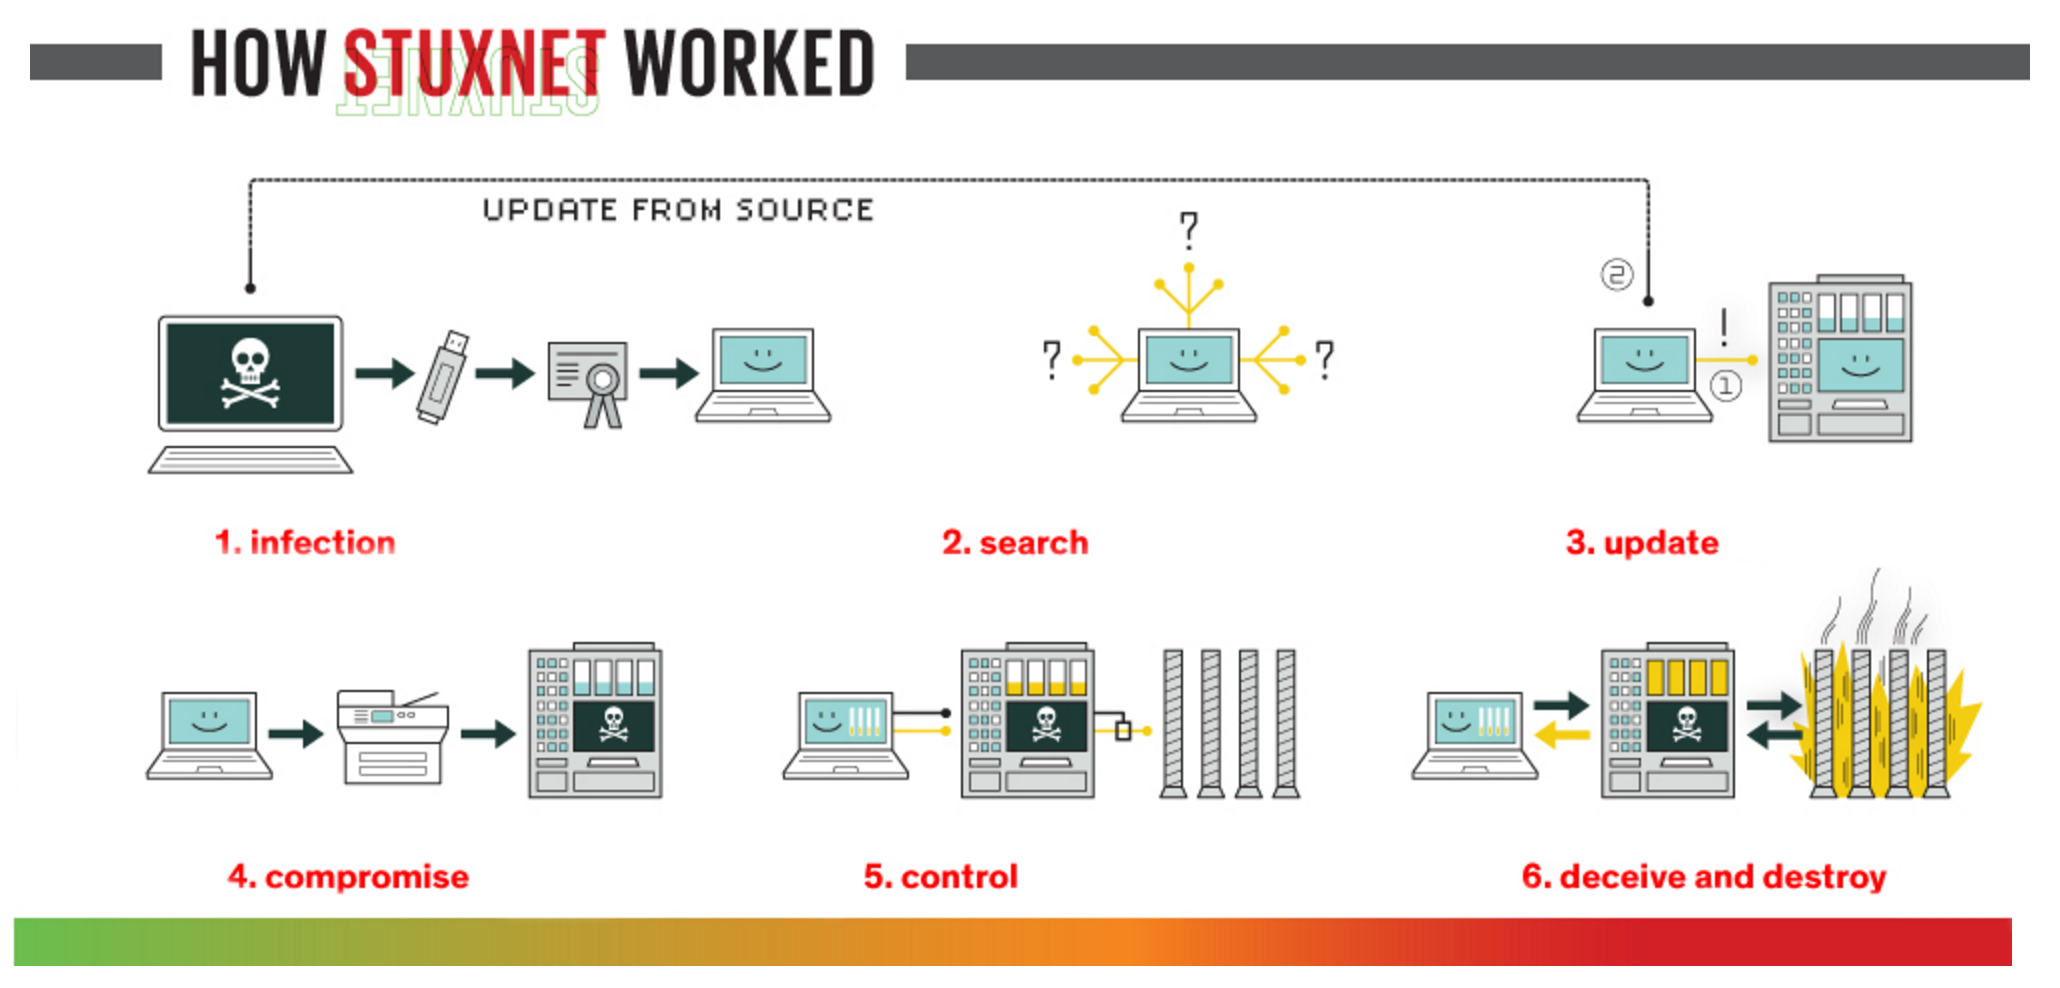
\includegraphics[scale=0.3,cfbox=blue_slides 1pt 0pt]{imgs/stuxnet_hsw.png}
	\end{figure}
\end{frame}

\begin{frame}{Un caso esemplare di attacco: Stuxnet}
	\begin{enumerate}
		\item \textbf{\color{blue_slides}Infection}: Entra nel sistema attraverso il collegamento di una penna USB e procede con l’infettare tutte le macchine su cui gira Windows (elude sistemi di automated-detection) %grazie a un certificato digitale che lo fa sembrare affidabile
		\pause
		\item \textbf{\color{blue_slides}Search}: Verifica se una macchina è parte del sistema di controllo industriale creato da Siemens
		\pause
		\item \textbf{\color{blue_slides}Update}: Se il sistema è quello target, il worm accede ad Internet per scaricare una versione più recente di se stesso
		\pause
		\item \textbf{\color{blue_slides}Compromise}: Compromette i controllori logici del sistema target %sfrutta la vulnerabilità zero-day
		\pause
		\item \textbf{\color{blue_slides}Control}: Spia le operazioni del sistema target ed utilizza le informazioni raccolte per prendere il controllo delle centrifughe %portandole al deterioramento
		\pause
		\item \textbf{\color{blue_slides}Deceive \& Destroy}: Fornisce informazioni fittizie ai controllori assicurandosi che non si accorgeranno del problema
	\end{enumerate}
\end{frame}

\begin{frame}
  \frametitle{Definire la sicureza}
  	\begin{figure}[h] 
		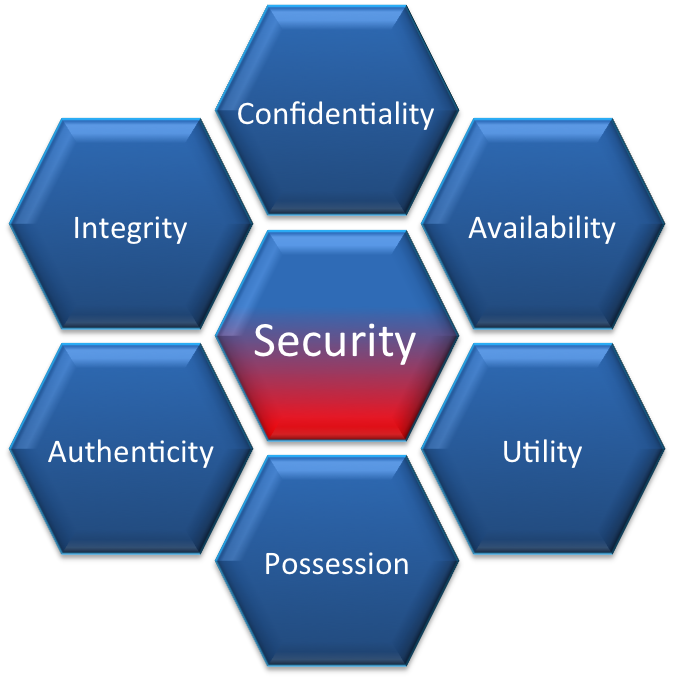
\includegraphics[scale=0.4]{imgs/hexad.png}
		\caption{Parkerian hexad}
	\end{figure}
\end{frame}

\begin{frame}
  \frametitle{Definire la sicurezza}
  \begin{itemize}[<+- | alert@+>]
  \item \textit{Confidentiality}
  	\begin{itemize}
  		\item Dati confidenziali $\rightarrow$ se noti, potrebbero causare danni alla sicurezza delle operazioni di tutto il sistema
  		\item Informazioni ricavate dal lavoro delle componenti della Smart Grid
  		\item Dati personali dei clienti $\rightarrow$ garantire la \textit{privacy}
  		\item Informazioni aziendali
  		\item Punti che introducono rischio: locazioni di memoria e meccanismi di trasmissione dati
  		\item Soluzioni: cifratura dei dati e controllo degli accessi
  	\end{itemize}
  \end{itemize}
\end{frame}

\begin{frame}
  \frametitle{Definire la sicurezza}
  \begin{itemize}[<+- | alert@+>]
  \item \textit{Integrity}
  	\begin{itemize}
  	\item Abilità del sistema di evitare che le informazioni siano modificate da persone o da sistemi non autorizzati
  	\item Mancanza di integrity $\rightarrow$ il sistema riceve dati non accurati $\rightarrow$ instabilità della Smart Grid
  	\item Punti che introducono rischio: componenti in cui si consente il passaggio dati da un sistema ad un altro
  	\item Soluzioni: \textit{auditing}, \textit{authorization}, \textit{nonrepudiation}, \textit{message-signing}
  	\end{itemize}
  \end{itemize}
\end{frame}

\begin{frame}
  \frametitle{Definire la sicurezza}
  \begin{itemize}[<+- | alert@+>]
  \item \textit{Availability}
  	\begin{itemize}
  	\item Capacità del sistema di compiere il lavoro che gli è stato assegnato, nel momento in cui se ne ha bisogno 
  	\item Punti che introducono rischio: qualsiasi sistema, rete, dispositivo che gestisce le comunicazioni e che si trova a dover effettuare l'inoltro di un comando da un’estremità del sistema ad un’altra
  	\item Soluzioni: tecniche di ridondanza
  	\end{itemize}
  \item \textit{Control (o Possession)}
  	\begin{itemize}
  	\item Capacità di controllare le informazioni che necessitano protezione
  	\item Mancanza di controllo dati $\rightarrow$  compromissione del sistema che li trasmette $\rightarrow$ provenienza delle informazioni non garantita $\rightarrow$ diminuzione dell'affidabilità di quest'ultime
  	\end{itemize}
  \end{itemize}
\end{frame}

\begin{frame}
  \frametitle{Definire la sicurezza}
  \begin{itemize}[<+- | alert@+>]
  \item \textit{Authenticity}
  	\begin{itemize}
  	\item Processo utilizzato per descrivere la certezza della provenienza
  	\item Assicurarsi che la fonte dei dati e i dati stessi siano autentici
  	\end{itemize}
  \item \textit{Usability (o Utility)}
  \begin{itemize}
  \item Assicurare che i dati siano utilizzabili
  \item Flusso di dati cifrato $\rightarrow$ garantisce la sicurezza ma rende difficile far sì che le informazioni siano utili
  \item Usabilità fornisce valore a livello aziendale $\rightarrow$ trattato come il requisito a più alta priorità
  \end{itemize}
  \end{itemize}
\end{frame}

\begin{frame}
  \frametitle{Building blocks}
  \begin{itemize}[<+- | alert@+>]
  \item \textit{Layered security model}
  \begin{itemize}
  \item Struttura ad anello 
  \item Comunicazione tra gli strati del sistema sicura
	  \begin{itemize}
  	\item Uno strato esterno non può avere libero accesso alle risorse presenti su uno strato più interno
  	\item Le richieste per le risorse non possono saltare gli anelli
  	\end{itemize}
  \item Assicurare che un fallimento in uno strato non abbia impatto nè in uno strato più basso nè in qualsiasi sistema dello stesso strato
  \end{itemize}
  \end{itemize}
    	\begin{figure}[h] 
		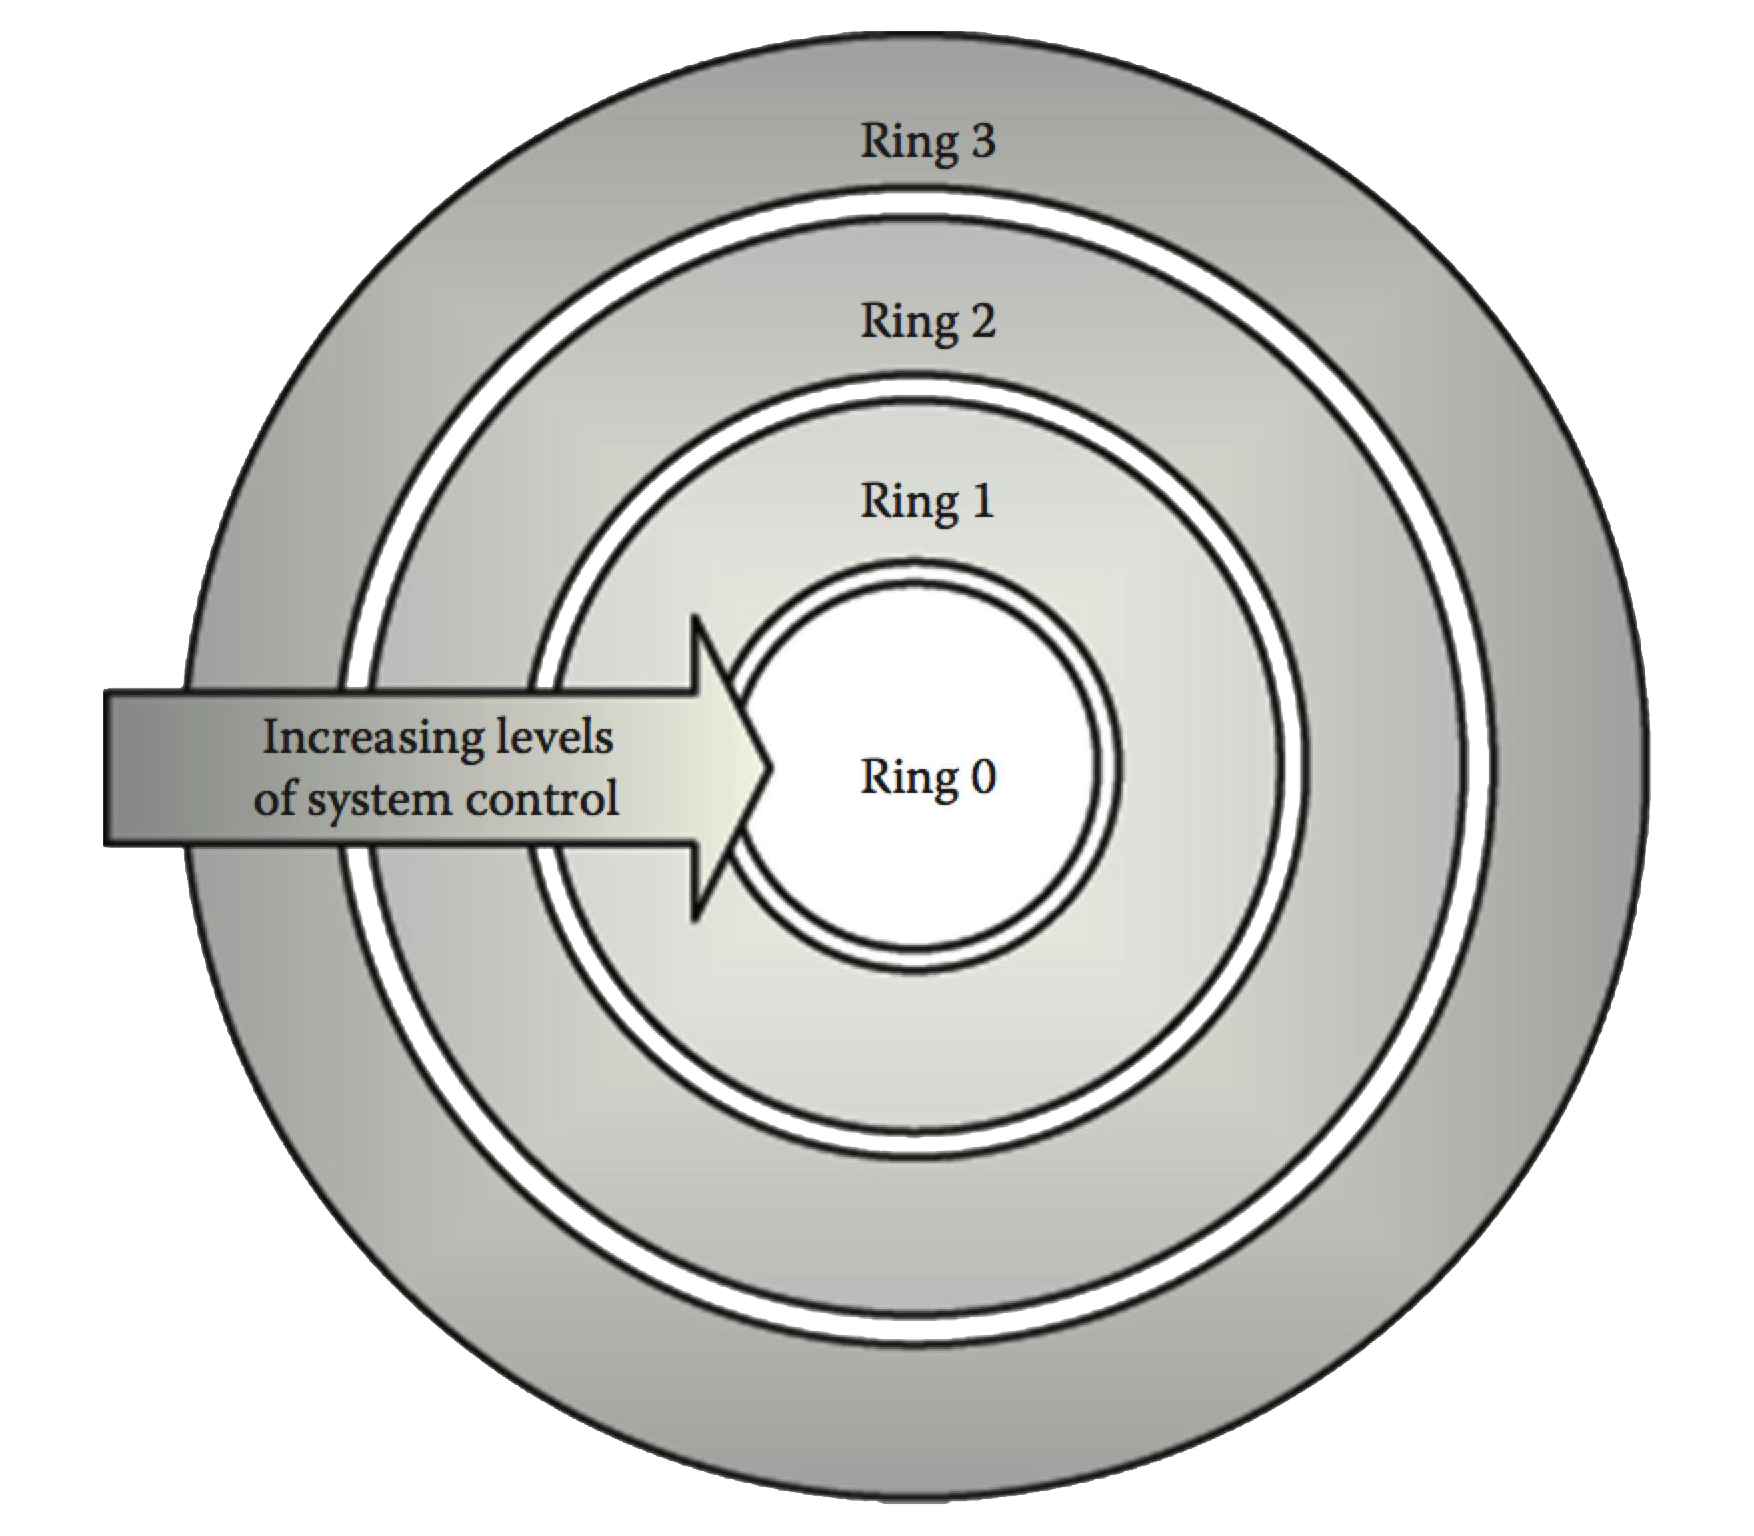
\includegraphics[scale=0.15]{imgs/ring.png}
	\end{figure}
\end{frame}

\begin{frame}
  \frametitle{Building blocks}
  \begin{itemize}[<+- | alert@+>]
  \item \textit{Authentication}
  \begin{itemize}
  \item Processo di verifica dell'identità di una persona o di un servizio che richiede l'accesso ad una risorsa
  \item Autenticazione non solo per l'utente ma anche tra sistemi, processi o componenti hardware
  \end{itemize}
 \item \textit{Authorization}
 	\begin{itemize}
 		\item Verifica di ciò che la persona o il servizio autenticato può fare all'interno del contesto del sistema
 	\end{itemize}
  \end{itemize}
\end{frame}

\begin{frame}
  \frametitle{Building blocks}
  \begin{itemize}[<+- | alert@+>]
  \item \textit{Auditing}
  \begin{itemize}
  \item Revisione periodica dell'efficacia dei meccanismi di sicurezza della Smart Grid
  \item Testing delle componenti essenziali per mettere in sicurezza le operazioni
  \end{itemize}
 \item \textit{Key management}
 	\begin{itemize}
 		\item Processo di gestione dell'emissione delle chiavi per utenti, applicazioni e dispositivi
 		\item Utilizzate per stabilire l'identità dell'utente e garantire l'integrità dei messaggi
 		\item Impiego di Public Key Infrastructure
 	\end{itemize}
  \end{itemize}
\end{frame}

\begin{frame}
  \frametitle{Building blocks}
  \begin{itemize}[<+- | alert@+>]
  \item \textit{Message integrity}
  \begin{itemize}
  \item Signing
  	\begin{itemize}
  	\item Messaggio inviato da un sistema ad un altro $\rightarrow$ autenticazione $\rightarrow$ autorizzazione $\rightarrow$ scambio di messaggi
  	\end{itemize}
  \item Nonrepudiation
    \begin{itemize}
  	\item Il mittente di un messaggio necessita di essere riconosciuto tramite una prova inconfutabile della sua identità
  	\end{itemize}
  \item Encryption
    \begin{itemize}
  	\item assicurarsi che un messaggio non possa essere letto da una persona o da un sistema che non sono i diretti destinatari dell’informazione
  	\end{itemize}
 	\end{itemize}
  \end{itemize}
\end{frame}

\begin{frame}
  \frametitle{Building blocks}
  \begin{itemize}[<+- | alert@+>]
  \item \textit{Network integrity}
  \begin{itemize}
  \item Firewall
  \item Rilevamento e prevenzione delle intrusioni
 	\end{itemize}
   \item \textit{System integrity}
     \begin{itemize}
  \item Protezione da malware
  \item Gestione della configurazione del sistema
  \item Validazione e testing
 	\end{itemize}
  \end{itemize}
\end{frame}

\begin{frame}
  \frametitle{Threats and Impacts: Consumer threats}
  \begin{itemize}[<+- | alert@+>]
  \item \textit{Minacce naturali}
	\begin{itemize}
	\item Venti, tempeste, tornadi e terremoti sono la causa di più del 50\% dei disturbi del sistema elettrico
	\item Eliminare totalmente i danni causati da tali calamità non è possibile
	\item Di critica importanza la definizione di programmi di aiuto in caso di incidenti
	\end{itemize}
  \end{itemize}
\end{frame}

\begin{frame}
  \frametitle{Threats and Impacts: Consumer threats}
  \begin{itemize}[<+- | alert@+>]
  \item \textit{Minacce da singoli o da organizzazioni}
	\begin{itemize}
	\item Ladri e stalker
	\item Hacker
	\item Terrorismo
	\item Governo
	\item Società di servizi, in particolare i lavoratori
	\end{itemize}
  \end{itemize}
\end{frame}

\begin{frame}
  \frametitle{Threats and Impacts: Consumer threats}
  \begin{itemize}[<+- | alert@+>]
  \item \textit{Impatti}
	\begin{itemize}
	\item Privacy del consumatore
		\begin{itemize}
		\item Gli smart meter raccolgono, tra i vari dati, anche informazioni personali degli utenti
		\item se tali dati giungono ad un hacker, potrà utilizzarli per scopi maliziosi
		\end{itemize}
	\item Impatto sull'availability
			\begin{itemize}
		\item Uno degli obiettivi principali della Smart Grid è rendere la corrente sempre disponibile
		\item Attacchi ai consumatori possono incidente sulla fornitura di corrente (alterazione di termostati, limitazione o impedimento di servizi d'emergenza) 
		\end{itemize}
	\item Impatto finanziario
				\begin{itemize}
		\item Corruzione di dati $\rightarrow$ emissione di bollette inaccurate
		\end{itemize}
  \end{itemize}
  \end{itemize}
\end{frame}

\begin{frame}
  \frametitle{Threats and Impacts: Utility companies threats}
  \begin{itemize}[<+- | alert@+>]
  \item \textit{Confidentiality}
  \begin{itemize}
	  \item Privacy del consumatore
	  \begin{itemize}
	  \item Attacco alla Web application della società che permette agli utenti di gestire i loro account
	  \item Analisi dello storico dei consumi di un utente per identificare azioni illegali
	  \end{itemize}
	\item Informazioni proprietarie
		\begin{itemize}
		\item Segreto aziendale $\rightarrow$ target degli hacker che pensano di poterlo vendere alle aziende competitrici
		\end{itemize}
 	\end{itemize}
 \end{itemize}
\end{frame}

\begin{frame}
  \frametitle{Threats and Impacts: Utility companies threats}
  \begin{itemize}[<+- | alert@+>]
  \item \textit{Integrity}
  \begin{itemize}
	  \item Frode
	  \begin{itemize}
	  \item Manomissione dello smart meter da parte degli utenti per sottostimare i loro consumi $\rightarrow$ bollette meno costose 
	  \item Modifica dei dati relativi alla produzione di energia di un consumatore $\rightarrow$ compensi maggiori
	  \end{itemize}
	\item Manipolazione dei dati dei sensori
		\begin{itemize}
		\item Simulare un guasto alla rete elettrica dell'intero vicinato $\rightarrow$ la società spende tempo e denaro per le riparazioni
		\end{itemize}
 	\end{itemize}
 \end{itemize}
\end{frame}

\begin{frame}
  \frametitle{Threats and Impacts: Utility companies threats}
  \begin{itemize}[<+- | alert@+>]
  \item \textit{Availability}
  \begin{itemize}
	  \item Clienti
	  \begin{itemize}
	  \item Un attaccante potrebbe connettersi allo smart meter di un utente, cambiare la password e spegnere la corrente in casa
	  \end{itemize}
	\item Organizzazioni
		\begin{itemize}
		\item Hacker che vuole danneggiare la società compiendo un \textit{Denial of Service attack}
		\item Ex dipendente di un'azienda che vuole vendicarsi del licenziamento
		\end{itemize}
	\item Manipolazione del mercato
		\begin{itemize}
		\item Hacker spinti da tornaconti economici, mettono le loro conoscenze a disposizione di un team non pratico del mestiere ma esperto di mercati finanziari 
		\item Ottenere significative quantità di denaro in poco tempo
		\end{itemize}
 	\end{itemize}
 \end{itemize}
\end{frame}
